\chapter{Evaluation} \label{cha:evaluation}

This chapter evaluates the outcome of the migration process. The pre-migration Image Manager is compared to the new serverless version from three different perspectives: a developmental perspective on the ease of local development, testing and deployment, a performance perspective on application performance, elasticity and robustness, and finally an economic perspective on the differences in hosting and operational cost. The latter two are approximated through a simple stress test and cloud provider pricing information, whereas the former is by nature less measurable and thus approached through a more qualitative and subjective assessment.

Serverless Image Manager's source code and stress test data can be found at \url{https://github.com/epiphone/image-manager}.

\section{Developer perspective}

From a development point of view the process of rewriting server application code into FaaS function handlers was found relatively simple. The same runtime environment (NodeJS v10) was used in both versions of the application and the deployment artifacts for both were built from the same codebase. The server application's code benefited from being modularized so that e.g. the server-specific request handling implementation was separated from image processing logic. These factors together enabled a high degree of code reuse when implementing FaaS functions. The source code of the image labeling function is presented in listing \ref{lst:labelerhandler} to exemplify how a comparatively small amount of boilerplate code is required to instantiate a new function: in this function the actual labeling logic is imported from a \textit{label} module which is shared with the server application.

\begin{lstlisting}[language=JavaScript,caption=Image labeler function handler,captionpos=b,label=lst:labelerhandler,showstringspaces=false,belowskip=2em,frame=tb,aboveskip=2em]
  import { Storage } from '@google-cloud/storage'
  import { getBucketFileLabels } from '../label'

  const gcs = new Storage()

  export async function labeler(data) {
    const labels = await getBucketFileLabels(data)

    return gcs
      .bucket(data.bucket)
      .file(data.name)
      .setMetadata({ metadata: { Labels: labels } })
  }
\end{lstlisting}

Developing and testing the functions locally was found more challenging, depending on function type. In case of the authorizer function local development was simple since the function exposes a synchronous HTTP API, behaving the same as a conventional server application. In that case a local development server could be used to mimic a deployed function without any mocking or test harnesses required. Developing the other functions locally was more difficult due to their event-driven invocation style which meant that the triggering cloud events would have to be replicated locally. Without any tooling in place to mock cloud events, it was found easier to deploy these functions to the cloud and develop against the actual deployed functions. While the deployment process is relatively fast, this did incur a degree of overhead in the development cycle: in larger projects it can be worth the investment to set up tooling for mocking parts of the cloud environment in order to avoid this overhead in local development. In short, local development of conventional serverful web applications can be more straightforward than corresponding serverless ones, but the problem is not one of invoking FaaS functions but of replicating cloud service dependencies.

Image Manager's function deployment process consists of four steps: building a deployment artifact from the shared codebase, compressing it into a zip file, uploading the zip to Cloud Storage and finally updating the function to use the new deployment artifact. All together the process takes about one minute. This is significantly faster than pre-migration deployment which consisted of building a Docker image, uploading the image to an image repository and restarting the VM with the new image. The serverless Image Manager also has the advantage in easily deploying multiple co-existing versions of a single function, which is useful for testing or rolling out new features.

Compared to the pre-migration application, the serverless Image Manager has a clear advantage in isolation and modularization. Having split the monolithic server application into four distinct functions means that individual deployment units are smaller and have fewer dependencies and are thus more comprehensible and maintainable. The functions are decoupled from each other which makes extending the application painless: adding a new image processing task for example amounts to creating a new function and attaching it to the Cloud Storage image upload event -- no changes in other functions are required. This level of isolation also grants the ability to deploy features independently.

From a service monitoring point of view, the two versions of Image Manager act similarly. Application logs are persisted in Google Cloud's logging service which can be used for searching and setting up monitoring alarms. Both versions offer insight into similar performance metrics through the cloud provider dashboard, with the serverless version benefiting from more granular per-function metrics. The serverful application has the advantage in that the image upload sequence is contained inside a single HTTP request, which makes tracing application behaviour easier. As the serverless application is by nature more distributed and event-driven the end-to-end flow of a particular task can be more difficult to follow. Distributed logging, i.e. adding a unifying correlation identifier to logs that originate from different services but belong to the same logical task, can be of use here and is provided as a service in some platforms, e.g. AWS X-Ray \parencite{awslambda0218}.

\section{Performance perspective}

The two Image Manager implementations' performance characteristics were evaluated through a simple stress test. The goal of the test was to understand how the applications behave under heavy load and to identify the upper limits of both application's performance capacity. The test was carried out by sending a gradually increasing number of image processing requests to the target application in a simulation of a steadily increasing influx of user activity, using the Python-based load testing tool Locust. The authentication step was omitted from the test in order to focus on the resource-intensive parts of the application i.e. image processing. For comparability's sake both the serverful application's VM and each serverless function was allocated the same resources of a single CPU and 1024MB of memory. In order to minimize network delays and traffic costs the tests were ran on a separate VM deployed on the same Google Cloud region as both applications.

The serverful application's stress test results are plotted in figure \ref{fig:serverfulStressTest}. The figure presents the number of all requests, number of error responses and the average response time during the 11-minute test period. Analyzing the results shows how response times initially stay below four seconds until at around 300 cumulative requests, after which they start climbing up to 14 seconds or more. Moreover the initial curve on the number of total requests evens out into linear growth which indicates that the server is unable to cope with the increasing request rate, maxing out at around 3 requests per second. Eventually after 600 cumulative requests we observe a sharp spike in error responses due to server resource exhaustion. At this point the server application becomes non-responsive as most requests resolve either in server error or connection timeout.

\begin{figure}[h]
  \centering
  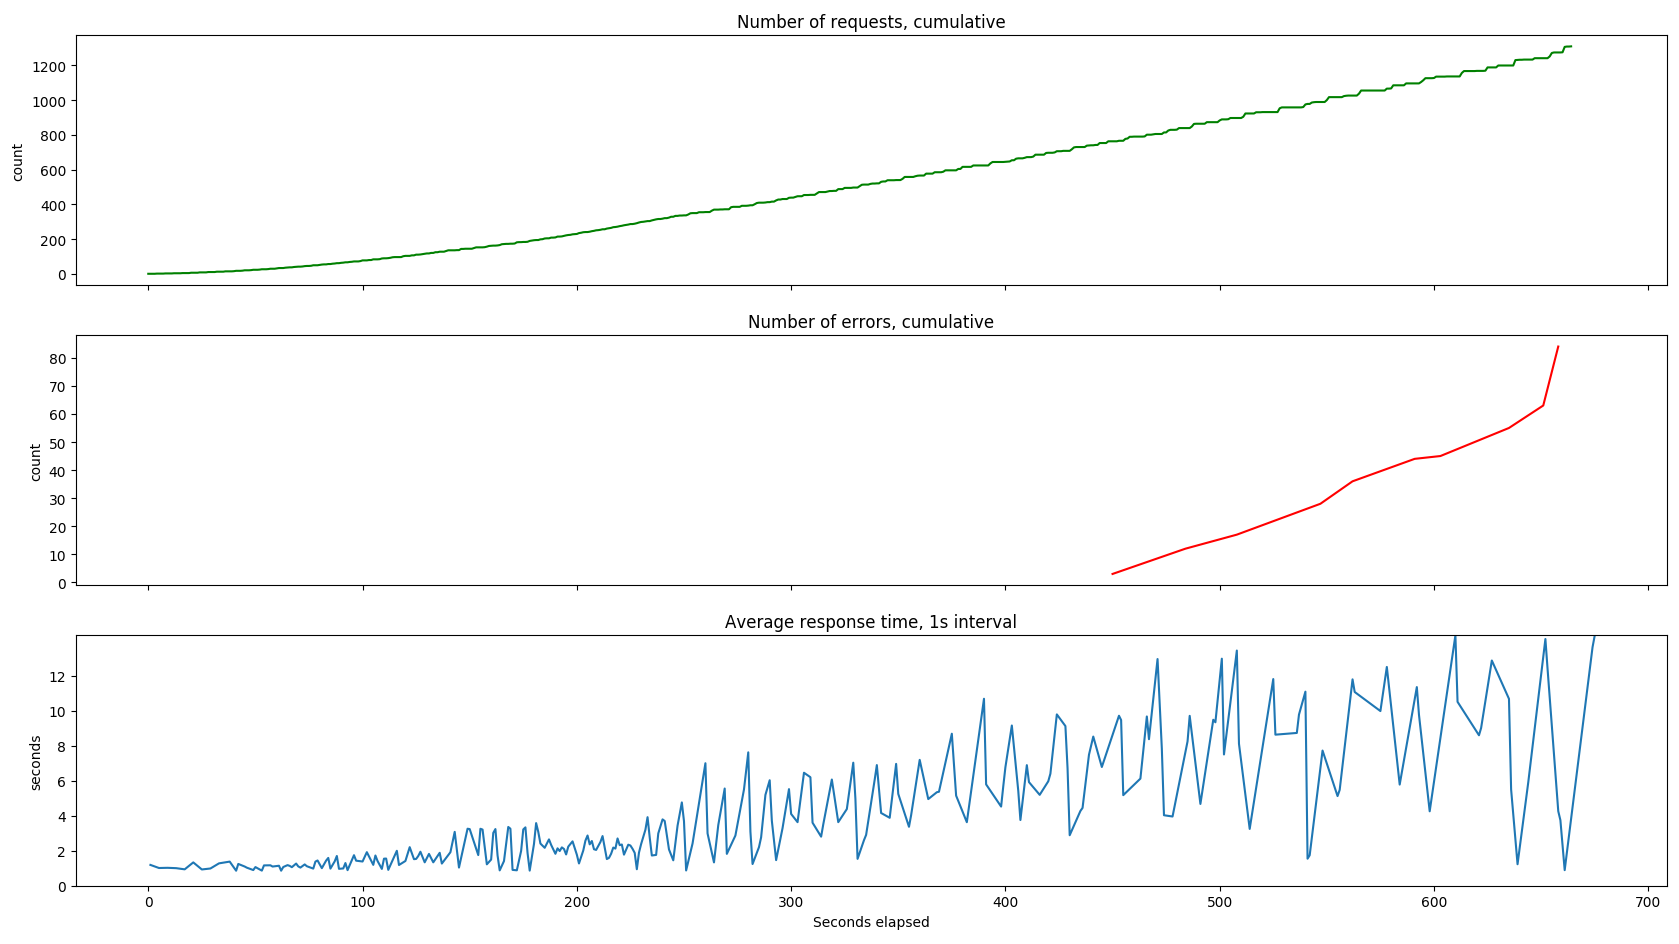
\includegraphics[width=0.75\textwidth]{serverful-load-test.png}
  \caption{Serverful Image Manager stress test results}
  \label{fig:serverfulStressTest}
\end{figure}

Running the same stress test against the serverless application yields differing results. Figure \ref{fig:serverlessStressTest} plots platform metrics captured during the test run, including the total function invocation rate per second, number of active instances per function and mean execution duration per function. First of all we observe the function invocation rate growing in tandem with the stress test's gradually increasing request rate. This is an expected outcome of the Event Processor pattern: as more images are uploaded to Cloud Storage, more processing tasks get triggered. The second chart illustrates the FaaS platform adapting to the growing invocation rate: an increasing number of function instances are spun up to handle invocations in parallel. While the sum of all of active instances peaks at around 100 we observe variance in scaling behaviour between the three functions, as the CPU-intensive LQIP rendering function scales up faster than the other two. Due to this scaling behaviour function execution durations stay constant while invocation rate grows from 0 to 60 per second, as plotted in the third chart. Interestingly the chart indicates slightly higher execution durations in the beginning of the test, which could be an indication of either function cold starts or the FaaS platform's underlying scaling strategy. With no sign of any performance degradation the test was aborted after 10 minutes.

\definecolor{gcpgreen}{RGB}{0,120,106}
\definecolor{gcporange}{RGB}{255,87,34}
\definecolor{gcpred}{RGB}{233,30,99}
\definecolor{gcpblue}{RGB}{159,171,228}

\begin{figure}[h]
  \centering
  \begin{subfigure}[b]{0.75\textwidth}
      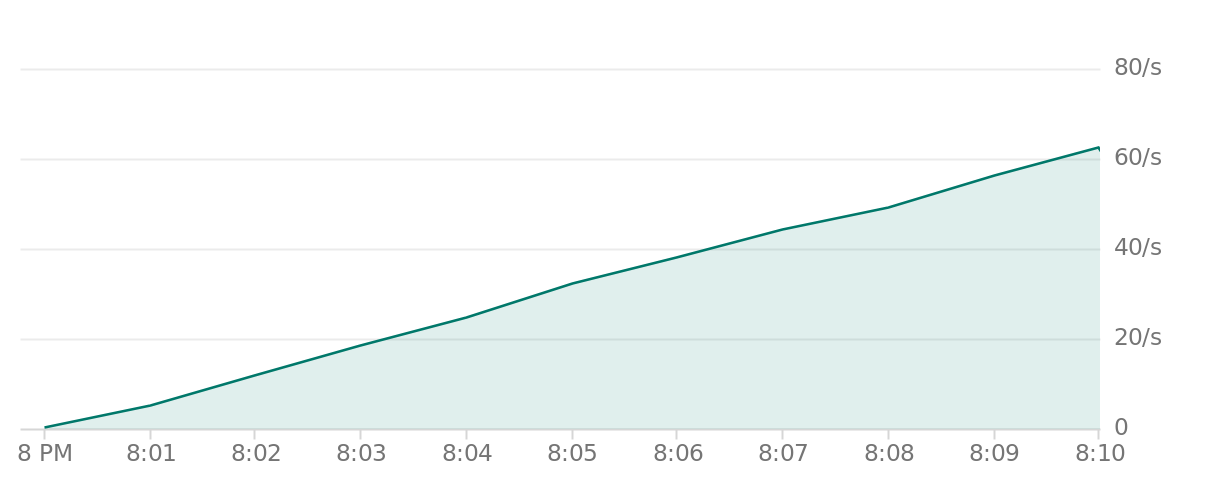
\includegraphics[width=\textwidth]{cloud-functions-invocations-per-second.png}
      \caption{Invocations per second, sum of all functions}
  \end{subfigure}

  \begin{subfigure}[b]{0.75\textwidth}
      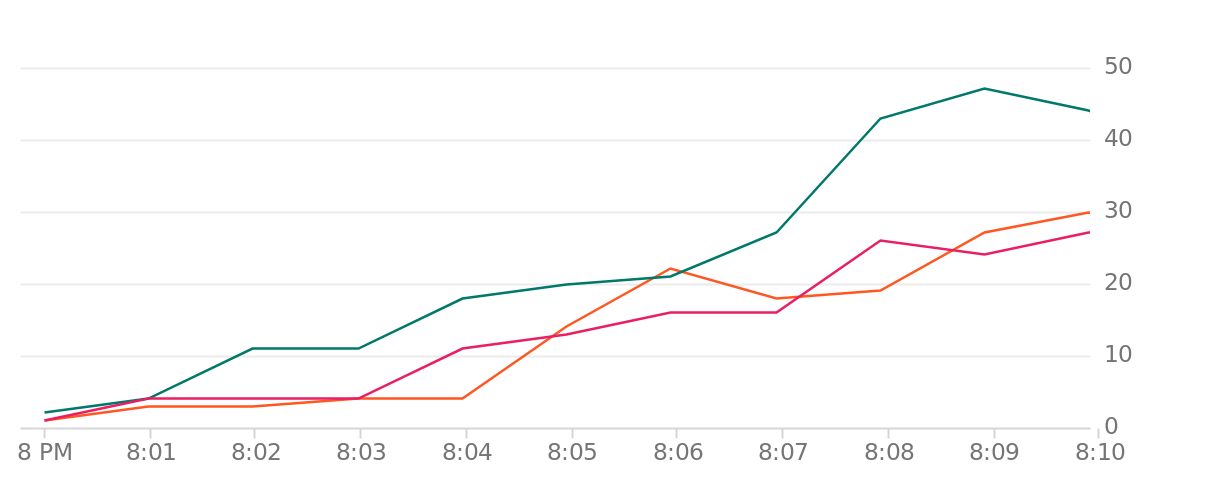
\includegraphics[width=\textwidth]{cloud-function-active-instances.png}
      \caption{Active instances per function ({\color{gcpgreen}LQIP}, {\color{gcporange}resizer}, {\color{gcpred}labeller})}
  \end{subfigure}

  \begin{subfigure}[b]{0.75\textwidth}
      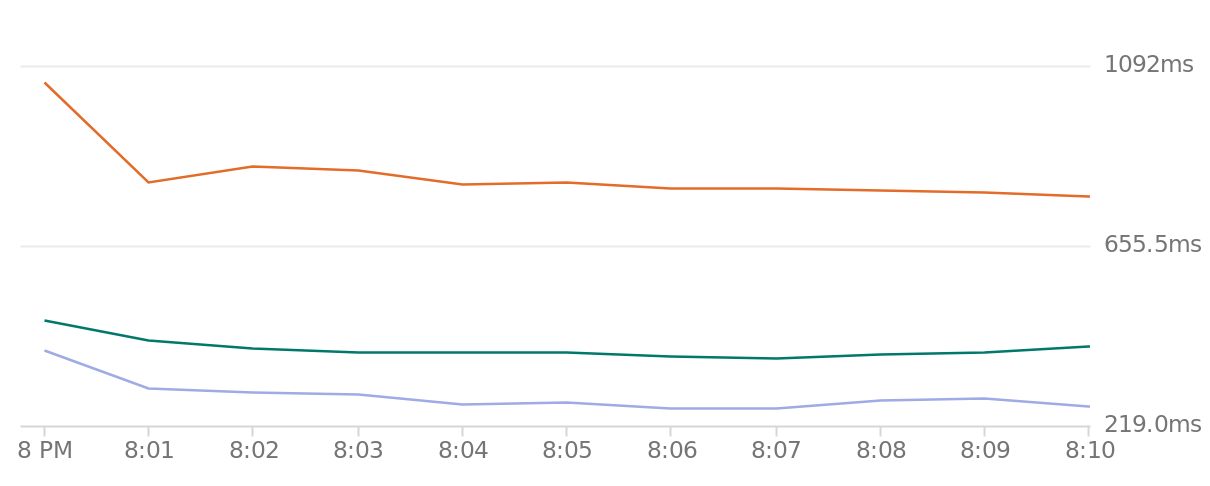
\includegraphics[width=\textwidth]{cloud-function-execution-times-mean.png}
      \caption{Mean execution times per function ({\color{gcporange}LQIP}, {\color{gcpgreen}labeller}, {\color{gcpblue}resizer})}
  \end{subfigure}
  \caption{Serverless Image Manager stress test results}\label{fig:serverlessStressTest}
\end{figure}

Overall the two Image Manager implementations perform quite differently performance-wise, as expected. The serverful application's response times stay in the range of a few seconds until service resources are exhausted and rise sharply after that along with the error rate. The serverless application on the other hand adapts to increasing load with constant execution durations, presumably until the platform's concurrency limit is reached. While server response times and function execution durations are not directly comparable (the latter lacks image upload and event propagation latencies) they do manage to convey the drastic difference in elasticity.

The serverless Image Manager's elasticity, while mostly beneficial, points towards the necessity of protecting any less elastic downstream services with something like the Throttler pattern in order not to overwhelm them. The results also demonstrate the efficiency of the Bulkhead pattern's granular deployment units as the LQIP rendering operation can scale independently without allocating redundant resources elsewhere to the system.

As for the problem of cold starts, an initial delay in image processing was deemed acceptable and did not thus necessitate the Function Warmer pattern. The pattern can be useful in case of synchronously invoked functions such as the authorizer function where any delay leaks to the consumer and potentially blocks the user interface. Drawing from that, another workaround over the cold start problem is to design ``optimistic'' clients that immediately update the user interface after function invocation instead of waiting for a response.

\section{Economic perspective}

Evaluating the two implementations from an economic perspective, the simplest metric to start with are the respective hosting costs. First of all any Cloud Storage and Cloud Vision API costs can be ignored as they are identical in both implementations and thus do not tip the scale either way. The reCaptcha API is a free service so it is similarly ignored. As for networking, no charges are incurred since incoming traffic (image upload requests) is free and outgoing traffic to provider services passes through internal networks free of charge.

In case of the serverful Image Manager hosting expenses consist solely of the VM, which is priced at \$18.3 per month for 1 CPU and 1GB of memory. Using the maximum capacity of 3 requests per second (or 7,776,000 requests per month) established in the stress test, we arrive at a per-image transformation cost of \$0.0000023534. This number represents a hypothetical best-case scenario of a constant 100\% utilization rate. In actuality lower utilization in form of any idle periods translates into a higher cost per image: 50\% utilization doubles the per-image cost, 10\% utilization means 10x the per-image cost and so on. Conversely any load above maximum capacity renders the service unusable. This single-VM configuration also does not have any form of redundancy in the sense that VM malfunction or restart immediately results in service downtime. A more realistic setup that achieves minimal robustness could consist of an additional failover instance and a load balancer sharing traffic between the two instances. This increases hosting costs to \$72.4 per month: 2 instances at \$18.3 each, load balancer forwarding rule at \$18 and incoming traffic cost of \$17.8 per month assuming an average image size of 300KB. \parencite{google18cloudFunctions}

As for the serverless Image Manager, a single image processing operation consists of 3 function invocations and on average a total of 1600 milliseconds of execution time (see figure \ref{fig:serverlessStressTest}). With Cloud Functions pricing of \$0.0000004 per invocation and \$0.00000165 per 100ms of execution on a 1024MB memory allocation, price per image adds up to \$0.0000276. Hence operating at the serverful Image Manager's maximum capacity of 3 requests per second for a month costs \$214.6 which is almost 12 times the cost of the serverful implementation. Therefore in case of Image Manager, a VM-based implementation operating at a constant 100\% utilization rate is by an order of magnitude cheaper to host than a serverless implementation. This is consistent with the level of service abstraction: renting a VM presumably incurs fewer costs to the cloud service provider than operating a fully-managed FaaS platform, so the price per CPU cycle should be higher for FaaS consumers. \parencite{google18cloudFunctions}

One way to optimize the serverless Image Manager's hosting costs would be by adjusting function memory allocation. For example the labeling function only uses on average 90MB of its 1024MB memory allocation. Reducing this down to the minimum 128MB allocation would reduce the above monthly cost to \$170.5 -- although since CPU allocation decreases alongside memory allocation this could in turn lead to longer execution duration. It is therefore necessary to experiment with real workloads to find out the optimal function size.

Determining which implementation is more economical depends ultimately on traffic scale and shape. Unlike the serverful implementation, the serverless price per image stays constant regardless of request rate. This extends down to the point of being free in case of no traffic. Thus while the serverful implementation is markedly cheaper in case of steady traffic that consistently utilizes the whole VM, the serverless one does better with bursty workloads scattered between idle periods. This is in accordance with the earlier notion that ``from a cost perspective, the benefits of a serverless architecture are most apparent for bursty, compute intensive workloads'' \parencite{baldini17currentTrends}. Aside from infrastructure costs it's worthwhile to consider the potential savings in operations, as FaaS requires less time expenditure on load estimation, scaling configuration and other system administration work than a VM-based solution. Also as discussed above, the more granular serverless Image Manager was found easier to extend, package and deploy than the monolithic serverful one which makes iteration and experimentation cheaper and can thus help to reduce time to market.
